\chapter{Recall}
\section{Saving the State}
To be able to recall past states a system needs to be in place that saves
parameters periodically. Every 100 frames a new `snapshot' of the state is
generated; this is an element in a JSON tree. Given the program is running at
around 60Hz (it is, however, not fixed) this means that approximately every 1.6
seconds the state is saved.

However, if we left the program running memory use would grow, so when saving
the state the program should check to see if it's changed or not. This has the
effect of compressing time neatly because you can interact with the program,
then step away and come back, begin interaction again and still be able to use
the recall as if there was no large gap between times.

The naive implementation of this is to create a JSON object that looks something
like this:

\begin{lstlisting}[language=javascript]
{
  "seed": 230128038,
  "uuid": 102830128,
  "elements": [
    {
      "x": 28,
      "y": 0,
      "z": 0,
      "noiseLevel": 0.4,
      "gridSpacing": 0.3
    },
    {
      "x": 31,
      "y": 10,
      "z": 0,
      "noiseLevel": 0.4,
      "gridSpacing": 0.3
    }
  ]
}
\end{lstlisting}

But, this approach of only using an array doesn't work, as when you `rewind'
you're branching from the progression that is ahead in the array. If
you only insert at the end of the array then this history gets mixed up leading
to a mess of non-chronological states.

So to fix this, a method using a tree should be devised. Each time you `rewind'
the tree should create a new branch from which you can begin control and
generate state elements in that branch. To do this I used the library 
\verb|Data-Tree|. This helps manage the tree structure by using references and
can export and import the structure to and from JSON. The library also provides
methods to search and traverse the tree, operating on each node.

Exporting the tree to a file is then simple, create a method that exports the
JSON tree and downloads it to the computer, the filename can be used to store
the seed. This works by creating a blob (binary large object), URL to the blob
and then a link element that downloads the JSON file, then using JavaScript to
click the link and finally removing the link.

\section{Drawing and Interaction}
Drawing the tree to the screen requires traversal. If we use depth-first
traversal we can work out where a new branch is formed by checking if the depth
of the node is the previous node's depth plus one. Then we can simply move down
and draw a point. If not, we branch, however it becomes more complicated; at
every node, we store the $(x,y)$ values into a JSON object with the key being the
node's unique key. Then when we see that the tree has branched we can find the
parent node (\verb|Data-Tree| stores this) and set the $y$ value to this and the
$x$ values increase by two times the diameter of the point. We then also need
to draw a line from the new branch's first node to the point where it branches,
this can be done by simply recalling the $x$ value of the parent node. Finally,
the most recent node is coloured red. In the end, it looks like this:

\begin{figure}[H]
    \centering
    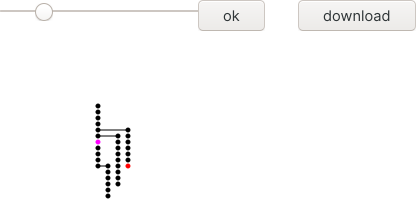
\includegraphics[width=.2\textwidth]{tree}
    \caption{}
\end{figure}

To interact with the tree, each point is modelled as a button. These buttons
have a \verb|display()| method that checks if the mouse is hovering and then
draws a point. The point becomes twice the size if hovered and uses the key of
the node to check whether to make itself red or not. The button can be used to
check when the mouse is clicked if the button is hovered at the time of clicking
and then the state can be loaded.

\begin{lstlisting}[language=JavaScript]
tree.traverser().traverseDFS(function(node) {
    if (prevDepth + 1 === node['_depth']) {
        b += treeButtonDiameter+1;
        values[node.data().key] = {'a':a, 'b':b};
        prevDepth = node['_depth'];
    } else {
        // get the parent node only when we branch
        parentNode = node.parentNode();
        b = values[parentNode.data().key].b;
        a += treeButtonDiameter*2;

        prevDepth = node['_depth'];
        
        // draw a line from the node to it's parent's
        push();
        strokeWeight(1);
        values[node.data().key] = {'a':a, 'b':b};
        line(values[parentNode.data().key].a + (treeButtonDiameter/2), b, a,b);
        pop();
    }

    let currentButton = new TreeButton(a, b, node.data().key, 
                                             treeButtonDiameter);
    currentButton.display(logger.getIndex());
    buttons.push(currentButton);
});
\end{lstlisting}

\section{Recalling Parameters}
Recalling parameters is simple, when we know the key of the node to recall (from
the button that was clicked on) we can search the tree and then return the
values stored at that node. The program then sets each of the variables in the
main script to these values.

Importing a tree from JSON is similar, except we use \verb|Data-Tree| to import
the file into its data structure first and then load the state at the last node
that was imported. We also call \verb|noiseSeed(filename)| (with the
\verb|.json| stripped) to set the seed correctly.

\section{Limitations}
Since the state is only saved every 1.6 seconds but we want to have a 'fluid'
method of playback, we can use a linear interpolation between two values in the
tree. This can be found by letting the user choose a non-integer index and using
\verb|p5js|'s \verb|lerp| function. Pseudo-code:

\begin{lstlisting}[language=javascript]
let ceil = Math.ceil(index);
let floor = ceil - 1;
let ceilElement = tree[ceil];
let floorElement = ceil.parent();

let t = index - floor;
var state = {}
//create elements in an interstitial state using lerp
for (var key in ceilParams) {
    state[key] = lerp(ceilElement.params[key], floorElement.params[key], t);
}
\end{lstlisting}

This assumes that the user is moving linearly between states which
may be the case if they're just holding buttons down. Other methods of
interpolation could be considered, but for the increased computing cost of a
polynomial interpolation or spline interpolation and that users are
unlikely to be moving in a way that either of these methods could fit either.
For example, if the user decides to move back and forth between two steps there
is no way to recover that data. Ultimately the user's inputs will never be able
to be modelled by interpolation; this method however saves having to keep the
state every frame and is `good enough' to recall a previous state as likely the
user cannot remember the exact configuration anyway.

The problem in integrating this into the program however is the user interface,
with the current model in which each history element is represented as a button,
there is no way to have the user click on a partial value. This is included in
the report because it is a technique that could be used in the future with a
different interface design.
